\documentclass{beamer}
\usepackage{graphicx}
\def \sarccontrib {{\bf SARC contribution}}
\newsavebox\myv

\begin{document}
\title{Performance Analysis and Optimization of C++ Standard Libraries}
\author{Sebastian Pop, Aditya Kumar}
\institute{SARC: Samsung Austin R\&D Center}
\date{October 26, 2017}

\frame{\titlepage}

\frame{\frametitle{Agenda}
  \begin{itemize}
  \item C++ standard template libraries
  \item software performance analysis
  \item improvements to libc++ and libstdc++ performance
  \end{itemize}
}

\frame{\frametitle{C++ Standard Template Libraries}
  \begin{itemize}
  \item STL is easy to use
    \begin{itemize}
    \item standard interface: portable
    \item easy to change data types: list, vector, deque, map, etc.
    \item easy to change algorithms: iterators
    \end{itemize}
  \item complexity specified by standard
  \item performance left to implementation
  \end{itemize}
}

\frame{\frametitle{Performance of STL implementations}
  \begin{itemize}
  \item performance and memory usage depend on
    \begin{itemize}
    \item implementation: libc++ vs. libstdc++ vs. MSVC, etc.
    \item container type
    \item inefficiencies in implementations
    \end{itemize}
  \item always analyze software performance to validate your choice
  \end{itemize}

  \begin{figure}
    \caption{Size in bytes of empty containers on x86\_64}
    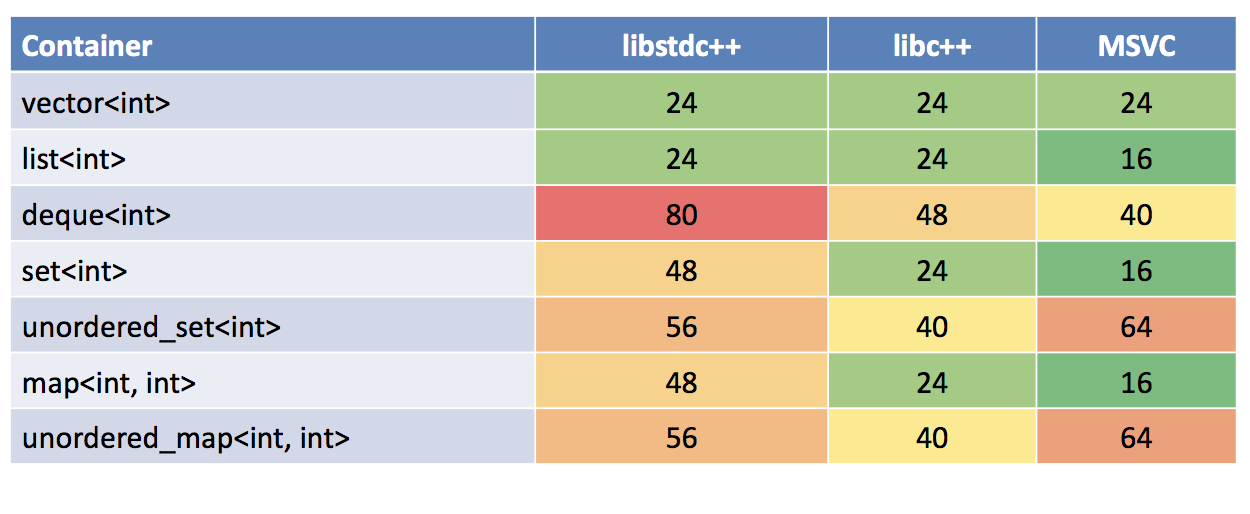
\includegraphics[width=\textwidth]{container_size.png}
  \end{figure}
}

%% \frame{\frametitle{Uses of STL implementations}
%%   Why are STL libs not used as much as intended? / expected?
%%   \begin{itemize}
%%   \item c++ power users implement a lot of critical data structures
%%   \item libc++ is cold on Android system wide profiles
%%   \item we contributed several changes to improve performance of libc++ and
%%     libstdc++ implementations
%%   \end{itemize}
%% }

\frame{\frametitle{Software Performance Analysis}
  \begin{itemize}
  \item identify hot functions from execution profiles
  \item inspect hot path: unit-benchmarking
  \item identify resource utilization on hot path
  \end{itemize}
}

\frame{\frametitle{Profiling: identify hot path}
  \begin{itemize}
  \item linux-perf: cycles, instructions, HW counters
  \item valgrind: cachegrind (R/W/Instrs), callgrind
  \item oprofile
  \end{itemize}
}

\frame{\frametitle{Unit-benchmarking: inspect hot path}
  unit-benchmarking is unit-testing for performance
  \begin{itemize}
  \item set-up data structures in memory
  \item call hot function
  \item execute hot function until performance measures stabilize \footnote{https://github.com/google/benchmark}
  \end{itemize}
  \vspace{1cm}
  
  check performance of a single hot operation: less noise, keep focus
}

\frame{\frametitle{Analyze resource utilization on hot path}
  Inspect:
  \begin{itemize}
  \item source code, compiler IR, assembly code
  \item CPU usage, instructions used and their latencies
  \item memory bus and caches: loads/stores, spills, cache misses
  \end{itemize}
}

\frame{\frametitle{Improve Software Performance}
  \begin{itemize}
  \item eliminate unnecessary work
    \begin{itemize}
    \item call functionality from libc or libc++
    \item reduce bus traffic: vectorize loads and stores
    \item help compiler remove redundancies: attributes and inline
    \end{itemize}
  \item analyze performance of different implementations
    \begin{itemize}
    \item change data structures
    \item change algorithms
    \item change STL implementations
    \end{itemize}
  \item analyze trade-offs of caching previous results
    \begin{itemize}
    \item use more memory vs. less computation (and vice versa)
    \end{itemize}
  \end{itemize}
}


\frame{\frametitle{Our contributions to improve performance of libc++ and libstdc++}
  \begin{itemize}
  \item string to int value parsing: xsgetn in libc++
    \begin{itemize}
    \item replace byte by byte copy with call to libc memcpy
    \item important speedup on proprietary benchmark
    \end{itemize}
  \item std::string.find() in libc++ and libstdc++
    \begin{itemize}
    \item replace byte by byte compare with call to memchr and memcmp
    \item 12x speedup on std-benchmark {\footnote{https://github.com/hiraditya/std-benchmark}}
    \end{itemize}
  \item inline ctor/dtor
    \begin{itemize}
    \item shared\_ptr
    \item basic\_string
    \end{itemize}
  \item add attribute noreturn to non-returning functions
    \begin{itemize}
    \item \_\_locale, vector, deque, future, regex, system\_error, etc.
    \item important for compiler optimizations
    \item remove false positives in static analysis tools
    \end{itemize}
  \end{itemize}
}

\frame{\frametitle{std::sort (libc++)}
  \begin{itemize}
  \item Convert to introsort
  \item Sorting technique, which begins with quicksort and switches to heapsort after recursion reaches a threshold
  \item Worst case complexity of O(NlogN)
  \item Eliminate recursion
  \item Replaced memory intensive recursive calls with stack – std::stack uses std::deque, which uses std::algorithm
  \item Improved worst case time complexity by a factor of 10 – https://reviews.llvm.org/D36423

  \item quicksort with tail recursion elimination: quadratic worst case
  \item reimplemented as introsort: begin with quicksort, switch to heapsort
    when recursion depth goes beyond a threshold
  \item 16x speedup in the worst case (std-benchmark {\footnote{https://github.com/hiraditya/std-benchmark}})

  \end{itemize}
}

\frame{\frametitle{Issues with std::sort (libc++)}
\begin{figure}
    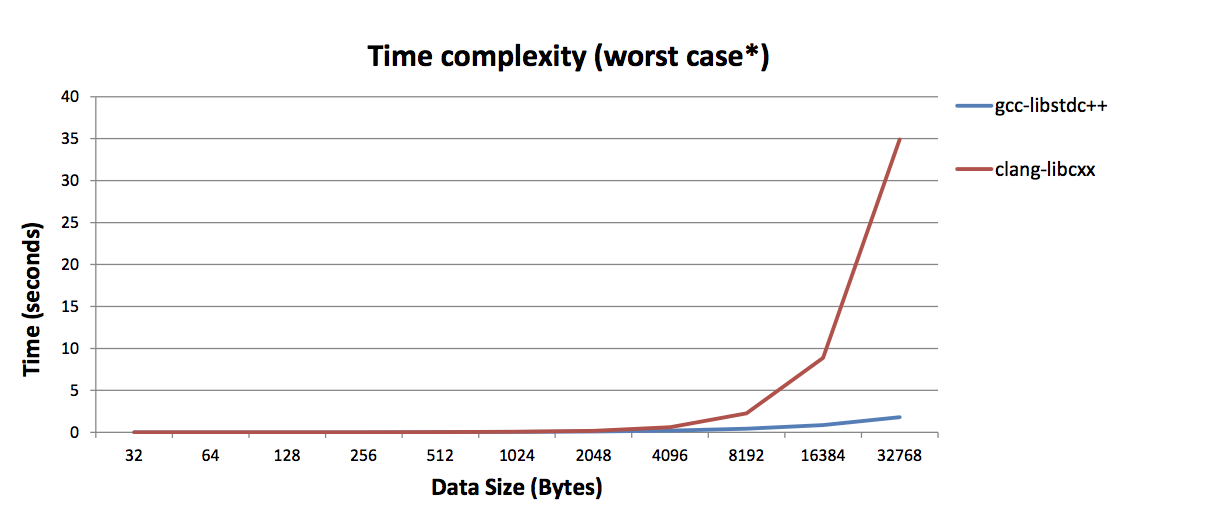
\includegraphics[width=\textwidth]{before.png}
\end{figure}
}

\frame{\frametitle{Sorting Results Plot (With std-benchmark)}
\begin{figure}
    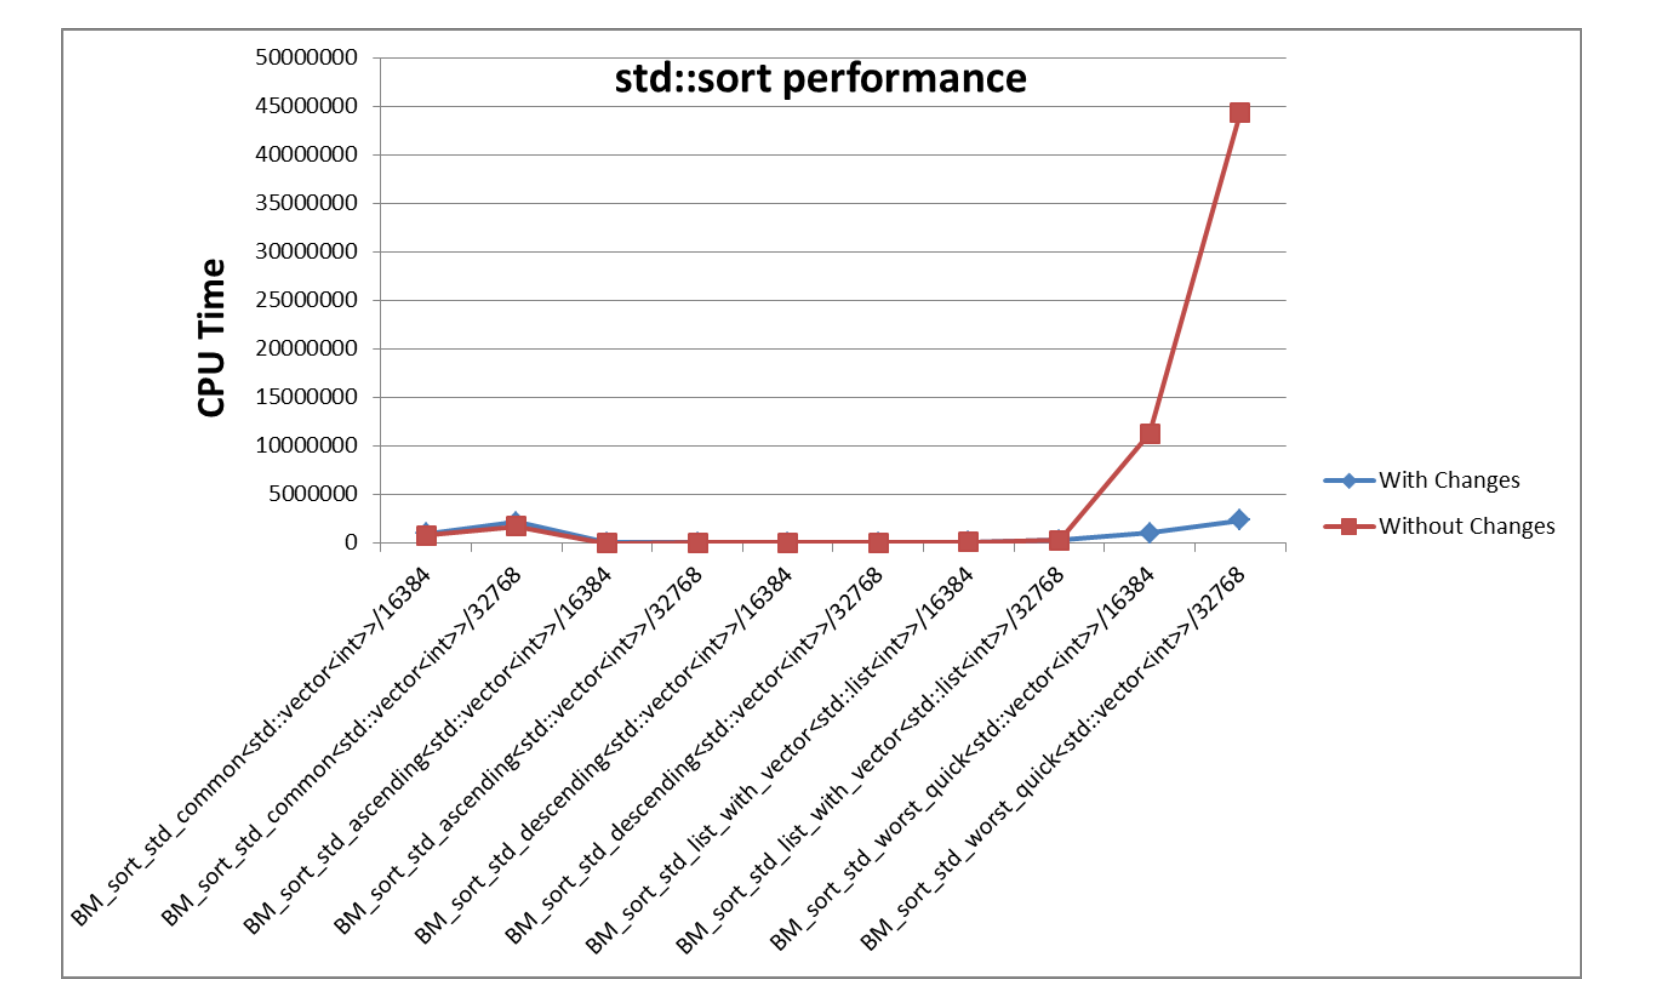
\includegraphics[width=\textwidth]{after.png}
\end{figure}
}



\frame{\frametitle{Lessons learned (containers) optimizing destructor of string}
\begin{figure}
    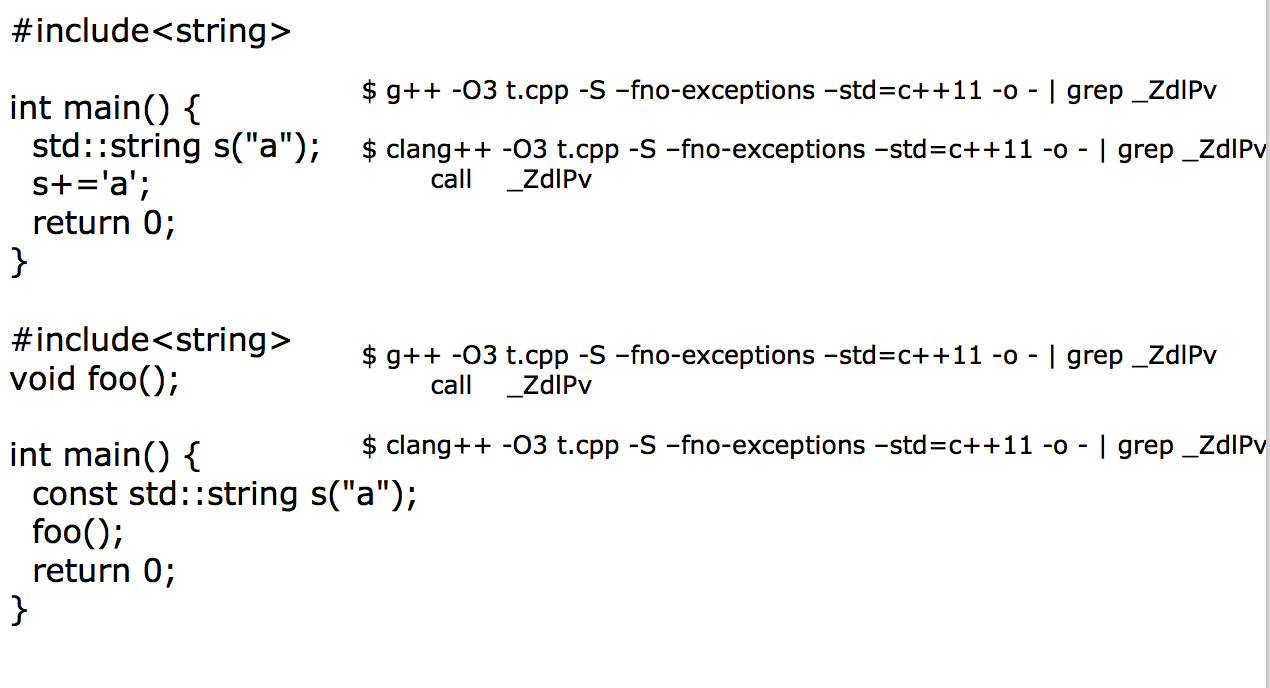
\includegraphics[width=\textwidth]{string.png}
\end{figure}
}


\frame{\frametitle{Annex}

}

\frame{\frametitle{Performance Analysis with Valgrind}
  \begin{itemize}
  \item {\ttfamily valgrind [--tool=memcheck]}
  \item {\ttfamily valgrind --tool=cachegrind}
    \begin{itemize}
    \item cache and branch simulator
    \item count read, write, and branch instructions
    \end{itemize}
  \item {\ttfamily valgrind --tool=callgrind}
    \begin{itemize}
    \item execution call graph
    \item visualization tool kcachegrind
    \end{itemize}
  \item {\ttfamily valgrind --tool=massif}
    \begin{itemize}
    \item how much heap and stack memory your program uses
    \item which parts of program allocate the heap memory
    \end{itemize}
  \end{itemize}
}

\begin{frame}[fragile]{Valgrind: Example -- SQLite}
  \begin{lrbox}{\myv}
    \begin{minipage}{\textwidth}
\begin{verbatim}
$ valgrind --tool=cachegrind ./sqlite_llvm <test.sql >/dev/null
[...]
--------------------------------------------------------------------------------
           Ir       I1mr   ILmr          Dr      D1mr    DLmr          Dw      D1mw    DLmw
--------------------------------------------------------------------------------
1,278,771,731 29,231,219 35,783 359,414,267 6,707,514 528,920 197,515,528 2,594,262 171,968  PROGRAM TOTALS
 
--------------------------------------------------------------------------------
         Ir      I1mr  ILmr         Dr      D1mr    DLmr         Dw    D1mw   DLmw  file:function
--------------------------------------------------------------------------------
363,052,233 7,560,087 3,122 97,707,865 1,084,529  77,197 44,505,055 217,826 29,838  src/sqlite3.c:sqlite3VdbeExec
 95,048,357    80,721   111 33,248,107    59,086   7,273 20,173,275      91      7  src/sqlite3.c:vdbeRecordCompareWithSkip
 68,045,026   695,509 1,144 14,883,933   114,698   1,918  5,525,733 272,507 19,249  src/sqlite3.c:balance
 56,713,554 1,101,002   276 18,416,705   683,914  21,085  3,453,665   1,947     25  src/sqlite3.c:sqlite3BtreeMovetoUnpacked
 45,344,891    59,660    66 13,589,490    66,121  18,775 12,795,281  59,451     86  src/sqlite3.c:sqlite3VdbeRecordUnpack
 36,550,248    47,192    94  9,615,816   217,845  11,567          0       0      0  src/sqlite3.c:cellSizePtr
 35,156,491 1,031,905   859  7,810,853   489,509   1,936  6,546,085 175,469 26,159  /build/glibc-2.19/malloc/malloc.c:_int_malloc
 34,402,967   219,015    40 12,316,213    31,625   1,007          0       0      0  src/sqlite3.c:vdbeRecordCompareInt
 31,287,698   269,233   121 10,094,976   398,015  57,982 10,094,976 797,005 41,768  /build/glibc-2.19/string/../ports/sysdeps/aarch64/memcpy.S:memcpy
 30,895,222 1,055,479   718  3,990,072    45,246     157  3,247,672   1,200     58  src/sqlite3.c:sqlite3VXPrintf
 29,633,734        87    87  6,992,348   510,654 147,437  1,945,350     292     14  src/sqlite3.c:vdbeSorterSort
 28,301,654 1,222,726   236  7,685,792   129,350     101  4,693,862  15,480     91  src/sqlite3.c:sqlite3BtreeInsert
 27,452,670   605,975   428  7,719,336   275,711   3,045  6,130,240   1,247    180  /build/glibc-2.19/malloc/malloc.c:_int_free
 26,152,338    93,230    53  5,107,641    26,455      59  3,502,857   6,705      2  src/sqlite3.c:sqlite3VdbeSerialGet
 21,638,172   664,339   241  7,621,765   197,153   7,033  5,509,634  12,988     53  src/sqlite3.c:sqlite3PagerAcquire
 19,904,842   811,018   134  6,875,142    93,695     809  4,223,778   6,655     72  src/sqlite3.c:insertCell
 17,184,877   622,046   254  5,927,277   207,045     101  3,228,818  13,564     78  src/sqlite3.c:pager_write
 16,511,495   127,072    29  5,189,327     7,164   1,105  2,358,785       0      0  src/sqlite3.c:serialGet
 14,566,464   347,254   101  5,076,192    68,798   4,135  3,972,672 131,226  9,179  src/sqlite3.c:moveToChild
 14,089,915   528,334   433  3,522,612   169,118     295      1,089      24     22  ???:???
 13,516,049   315,369    75  3,660,565    70,941     104  2,252,728   2,740     20  /build/glibc-2.19/malloc/malloc.c:malloc
 13,444,711   370,614    60  3,136,255    74,755  57,116  3,757,149       0      0  src/sqlite3.c:btreeParseCellPtr
 11,814,468   620,489   364  3,444,231   109,318     159  1,401,768  11,253      7  src/sqlite3.c:sqlite3VdbeHalt
  9,867,819   655,851   130  3,350,976    68,237      46  1,820,276  62,050     70  src/sqlite3.c:moveToRoot
  9,023,249   615,625   175  2,774,458    27,649      72  1,719,012     578      1  src/sqlite3.c:sqlite3VdbeMemGrow
  9,015,155   136,420   114  2,528,161    33,460      40  1,808,361      12      7  /build/glibc-2.19/nptl/pthread_mutex_lock.c:pthread_mutex_lock
  8,932,696   193,491    71  1,956,326    55,921      22  1,411,634       2      0  /build/glibc-2.19/nptl/pthread_mutex_unlock.c:__pthread_mutex_unlock_usercnt
  8,916,165    82,925    47  2,092,310         0       0  1,933,573   1,583      3  src/sqlite3.c:memjrnlWrite
  8,869,488   284,528    72  4,276,902   299,688   8,315  1,834,026   6,712     17  src/sqlite3.c:pcache1Fetch
  8,120,421   171,173   145          0         0       0  4,459,287 446,962 23,788  /build/glibc-2.19/string/../ports/sysdeps/aarch64/memset.S:memset
  7,759,659   338,888    58  2,364,882    24,321   1,308  1,624,112 104,416  1,631  src/sqlite3.c:sqlite3PcacheRelease
  6,799,934    97,805   282  2,068,211    38,793     684  1,555,697   3,672     11  src/sqlite3.c:sqlite3BtreeNext
  6,674,044    88,515   123  1,706,065     4,244      43  1,094,451       7      0  src/sqlite3.c:freeSpace
  6,536,765   760,083   320  2,119,849   121,314      85  1,091,200       0      0  src/sqlite3.c:sqlite3_step
\end{verbatim}
    \end{minipage}
  \end{lrbox}
  \resizebox{0.4\textwidth}{!}{\usebox\myv}
\end{frame}

\frame{\frametitle{Performance Analysis with Linux Perf}
  Two modes of operation:
  \begin{itemize}
  \item sum up all counters: {\ttfamily perf stat}
  \item record events: {\ttfamily perf record}
  \end{itemize}
}

\begin{frame}[fragile]{Linux Perf: Example -- SQLite}
  \begin{lrbox}{\myv}
    \begin{minipage}{\textwidth}
\begin{verbatim}
  $ perf stat ./sqlite_llvm <test.sql >/dev/null
 
 Performance counter stats for './sqlite_llvm':
 
       1045.856070      task-clock (msec)         #    1.000 CPUs utilized
                 1      context-switches          #    0.001 K/sec
                 0      cpu-migrations            #    0.000 K/sec
               809      page-faults               #    0.774 K/sec
     1,636,720,010      cycles                    #    1.565 GHz                     [83.16%]
       548,530,227      stalled-cycles-frontend   #   33.51% frontend cycles idle    [83.16%]
       218,991,051      stalled-cycles-backend    #   13.38% backend  cycles idle    [67.04%]
     3,385,841,295      instructions              #    2.07  insns per cycle
                                                  #    0.16  stalled cycles per insn [83.54%]
       709,436,490      branches                  #  678.331 M/sec                   [83.54%]
         2,586,354      branch-misses             #    0.36% of all branches         [83.17%]
 
       1.045918998 seconds time elapsed
\end{verbatim}
    \end{minipage}
  \end{lrbox}
  \resizebox{0.5\textwidth}{!}{\usebox\myv}
\end{frame}

\begin{frame}[fragile]{Linux Perf: Example -- 483.xalancbmk}
  \begin{lrbox}{\myv}
    \begin{minipage}{\textwidth}
\begin{verbatim}
$ perf record ./xalancbmk
$ perf report
  0.20 │629a84:   ldr    w9, [x0,#24]
 18.71 │629a88:   ldr    w8, [x1,#24]
 12.93 │629a8c:   cmp    w9, w8
  2.74 │629a90:   b.ne   629af8 <xalanc_1_8::XalanDOMString::equals
  2.00 │629a94:   ldp    x8, x10, [x0]
  2.43 │629a98:   cmp    x8, x10
  1.80 │629a9c:   ldp    x10, x12, [x1]
  1.03 │629aa0:   adrp   x11, 704000 <vtable for xalanc_1_8::ReusableArenaBlock+0x8>
  0.53 │629aa4:   add    x11, x11, #0xb08
  0.03 │629aa8:   csel   x8, x11, x8, eq
  1.33 │629aac:   cmp    x10, x12
  0.34 │629ab0:   csel   x10, x11, x10, eq
  1.78 │629ab4:   cbz    w9, 629b00 <xalanc_1_8::XalanDOMString::equals
  0.02 │629ab8:   ldrh   w11, [x8]
  4.02 │629abc:   ldrh   w12, [x10]
  3.75 │629ac0:   cmp    w11, w12
  1.03 │629ac4:   b.ne   629b08 <xalanc_1_8::XalanDOMString::equals
  1.16 │629ac8:   lsl    x9, x9, #1
       │629acc:   add    x8, x8, #0x2
       │629ad0:   add    x10, x10, #0x2
       │629ad4:   sub    x9, x9, #0x2
 10.18 │629ad8:   cbz    x9, 629b00 <xalanc_1_8::XalanDOMString::equals
  0.01 │629adc:   ldrh   w11, [x8],#2
 18.79 │629ae0:   sub    x9, x9, #0x2
  0.00 │629ae4:   ldrh   w12, [x10],#2
  9.22 │629ae8:   cmp    w11, w12
  5.11 │629aec:   b.eq   629ad8 <xalanc_1_8::XalanDOMString::equals
       │629af0:   mov    w0, wzr
       │629af4:   ret
  0.69 │629af8:   mov    w0, wzr
  0.09 │629afc:   ret
       │629b00:   orr    w0, wzr, #0x1
  0.10 │629b04:   ret
       │629b08:   mov    w0, wzr
       │629b0c:   ret
\end{verbatim}
    \end{minipage}
  \end{lrbox}
  \resizebox{0.5\textwidth}{!}{\usebox\myv}
\end{frame}

\end{document}
